\documentclass[12pt]{article}
\usepackage[margin=1in]{geometry} % set suitable margins
\usepackage{tikz}
\usepackage{circuitikz}
\usetikzlibrary{patterns}
\usetikzlibrary{arrows.meta, decorations.pathmorphing}
\usepackage{amsmath}

% Define colors
\definecolor{bluecolor}{RGB}{173,216,230} % Light blue
\definecolor{purplecolor}{RGB}{210,180,222} % Light purple
\definecolor{pinkcolor}{RGB}{255,182,193} % Light pink
\definecolor{orangecolor}{RGB}{252, 213, 180} % Light orange

\title{EMCH 354 HW 2 Solutions}
\author{Jacob Vaught}
\date{}

\begin{document}
\maketitle

\section*{Question \#1}
Determine the effective heat transfer coefficient, \( h_r \), resulting from radiation heat transfer if the surrounding temperature is \( 200^\circ C \) and the surface temperature is \( 50^\circ C \) with an emissivity of \( 0.8 \).
\begin{center}
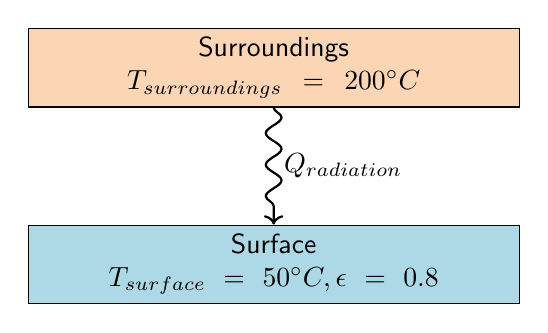
\begin{tikzpicture}[font=\sffamily]
    % Define the style for the surfaces
    \tikzstyle{surface} = [draw, fill=bluecolor, text width=6cm, minimum height=1cm, align=center]

    % Surface with lower temperature (receiving heat)
    \node[surface] (surface) at (0,0) {Surface \\ \( T_{surface} = 50^\circ C, \epsilon = 0.8 \)};

    % Surroundings with higher temperature (emitting heat)
    \node[surface, fill=orangecolor] (surroundings) at (0,2.5) {Surroundings \\ \( T_{surroundings} = 200^\circ C \)};

    % Radiation heat transfer arrows (pointing from the surroundings to the surface)
    \draw[->,thick, decorate, decoration={snake, amplitude=1mm, segment length=4mm, post length=1mm}] (surroundings.south) -- (surface.north)
        node[midway,right] {\( Q_{radiation} \)};
\end{tikzpicture}
\end{center}

\subsection*{Mathematical Solution}
The effective heat transfer coefficient due to radiation, \( h_r \), is calculated using the formula:

\[
h_r = \frac{\epsilon \sigma (T_1^4 - T_2^4)}{T_1 - T_2}
\]
\noindent
Where:
\begin{itemize}
    \item \(\epsilon\) is the emissivity of the surface.
    \item \(\sigma\) is the Stefan-Boltzmann constant (\(5.67 \times 10^{-8} \, W/m^2K^4\)).
    \item \(T_1\) is the absolute temperature of the surface.
    \item \(T_2\) is the absolute temperature of the surroundings.
\end{itemize}
\noindent
Converting the given temperatures from Celsius to Kelvin and substituting the values:

\[
T_{surface} = 50^\circ C = 323.15 \, K
\]
\[
T_{surroundings} = 200^\circ C = 473.15 \, K
\]
\noindent
The effective heat transfer coefficient, \( h_r \), is:

\[
h_r = \frac{0.8 \times 5.67 \times 10^{-8} \times (323.15^4 - 473.15^4)}{323.15 - 473.15}
\]
\noindent
Solving for \( h_r \), we find that it is approximately \( 11.86 \, W/m^2K \).



\section*{Question \#2}
A special-purpose oil flows at \(45.25 \, \text{kg/m}^2\text{s}\) inside a \(10 \, \text{cm}\)-long duct with rectangular cross section (\(1 \, \text{cm} \times 4 \, \text{cm}\)) that is heated electrically at a rate of \(100 \, \text{W/m}^2\) along the length direction. Given thermal properties are \(k = 0.139 \, \text{W/m-K}\), \(\rho = 854 \, \text{kg/m}^3\), \(c_p = 2120 \, \text{J/kg-K}\), and \(\nu = 4.1 \times 10^{-5} \, \text{m}^2/\text{s}\). Determine:
a) Mass flow rate, 
b) Volumetric flow rate, 
c) Bulk fluid velocity, 
d) Reynolds number, 
e) Convective heat transfer coefficient with \(Nu=4.36\), 
f) Temperature difference between wall and bulk fluid,  
g) Temperature difference between inlet and outlet, and 
h) Pressure drop gradient with \(Re \cdot Dh \cdot f = 73\).
\subsubsection*{Figure 1: 3D View of the Heated Duct}
\begin{center}
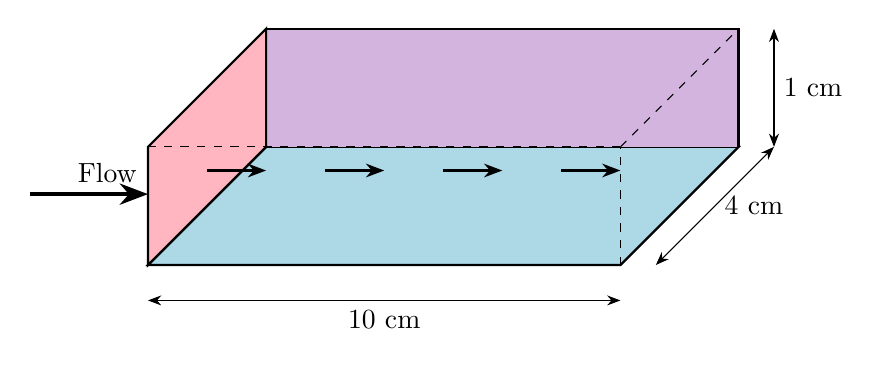
\begin{tikzpicture}[scale=1.5, >=Stealth]
    % Top side of the duct
    \fill[bluecolor] (0,0) -- (4,0) -- (5,1) -- (1,1) -- cycle;
    \draw[thick] (0,0) -- (4,0) -- (5,1) -- (1,1) -- cycle;
    
    % Side of the duct
    \fill[purplecolor] (5,1) -- (5,2) -- (1,2) -- (1,1) -- cycle;
    \draw[thick] (5,1) -- (5,2) -- (1,2) -- (1,1);
    
    % Front of the duct (visible part)
    \fill[pinkcolor] (0,0) -- (1,1) -- (1,2) -- (0,1) -- cycle;
    \draw[thick] (0,0) -- (1,1) -- (1,2) -- (0,1) -- cycle;
    
    % Dashed lines for the wireframe view
    \draw[dashed] (4,0) -- (4,1);
    \draw[dashed] (4,1) -- (4,1,-2.5);
    \draw[dashed] (4,1) -- (0,1);
    
    % Flow arrows on top side
    \foreach \x in {0.5,1.5,...,3.5}
        \draw[->,thick] (\x,0.8) -- ++(0.5,0);
    
    % Labeling the duct dimensions
    \draw[<->] (0,-0.3) -- node[below] {10 cm} (4,-0.3); % Length
        % Labeling the back
    \draw[<->] (4.3,0) -- node[right] {4 cm} (5.3,1); % Width
    \draw[<->] (5.3,1) -- node[right] {1 cm} (5.3,2); % Height

    % Labeling the flow
    \draw[->,ultra thick] (-1,0.6) -- (0,0.6) node[above left] {Flow};
\end{tikzpicture}
\end{center}


\subsubsection*{Figure 2: Heat Transfer View of the Duct}
\begin{center}
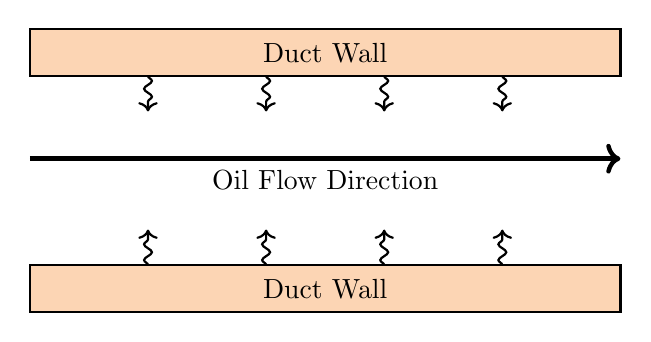
\begin{tikzpicture}[scale=1.5]
    % Define the thickness of the duct walls
    \newcommand{\ductthickness}{0.4}
    
    % Upper duct wall
    \fill[orangecolor] (0,1) rectangle ++(5,\ductthickness);
    \draw[thick] (0,1) rectangle ++(5,\ductthickness);
    
    % Lower duct wall
    \fill[orangecolor] (0,-1) rectangle ++(5,\ductthickness);
    \draw[thick] (0,-1) rectangle ++(5,\ductthickness);
    
    % Heat transfer arrows
    \foreach \x in {1,2,...,4}
        \draw[->, thick, decorate, decoration={snake, amplitude=0.5mm, segment length=2mm, post length=0.5mm}] (\x,0.8+\ductthickness/2) -- ++(0,-0.3);

    \foreach \x in {1,2,...,4}
        \draw[->, thick, decorate, decoration={snake, amplitude=0.5mm, segment length=2mm, post length=0.5mm}] (\x,-0.8+\ductthickness/2) -- ++(0,0.3);
    % Oil flow direction arrow
    \draw[->,fill=black,ultra thick] (0,0.3) -- ++(5,0) node[midway,below] {Oil Flow Direction};

    % Labels for the duct walls
    \node at (2.5,1+\ductthickness/2) {Duct Wall};
    \node at (2.5,-1+\ductthickness/2) {Duct Wall};
\end{tikzpicture}
\end{center}

\subsection*{Solution}
a) Mass flow rate:
\[ \dot{m} = \text{flow rate per area} \times \text{cross-sectional area} = 45.25 \, \text{kg/m}^2\text{s} \times 0.04 \, \text{m}^2 = 1.81 \, \text{kg/s} \]
\noindent
b) Volumetric flow rate:
\[ \dot{V} = \frac{\dot{m}}{\rho} = \frac{1.81 \, \text{kg/s}}{854 \, \text{kg/m}^3} = 2.12 \times 10^{-5} \, \text{m}^3/\text{s} \]
\noindent
c) Bulk fluid velocity:
\[ u = \frac{\dot{V}}{\text{cross-sectional area}} = \frac{2.12 \times 10^{-5} \, \text{m}^3/\text{s}}{0.04 \, \text{m}^2} = 0.05299 \, \text{m/s} \]
\noindent
d) Reynolds number:
\[ Re = \frac{uD_h}{\nu} \]
\[ D_h = \frac{2ab}{a+b} = \frac{2 \times 0.01 \, \text{m} \times 0.04 \, \text{m}}{0.01 \, \text{m} + 0.04 \, \text{m}} = 0.016 \, \text{m} \]
\[ Re = \frac{0.05299 \, \text{m/s} \times 0.016 \, \text{m}}{4.1 \times 10^{-5} \, \text{m}^2/\text{s}} = 20.68 \]
\noindent
e) Convective heat transfer coefficient:
\[ h = Nu \cdot \frac{k}{D_h} = 4.36 \times \frac{0.139 \, \text{W/m-K}}{0.016 \, \text{m}} = 37.88 \, \text{W/m}^2\text{K} \]
\noindent
f) Temperature difference between wall and bulk fluid:
\[ \Delta T = \frac{q}{h} = \frac{100 \, \text{W/m}^2}{37.88 \, \text{W/m}^2\text{K}} = 2.64 \, \text{K} \]
\noindent
g) Temperature difference between inlet and outlet:
Given the heat transfer per unit area (\( q \)) and the wetted perimeter (\( P \)), the temperature difference can be calculated by:
\[ \Delta T_{in-out} = \frac{q \cdot P}{\dot{m} \cdot c_p} \]
\[ \Delta T_{in-out} = \frac{100 \, \text{W/m}^2 \cdot 0.10 \, \text{m}}{1.81 \, \text{kg/s} \cdot 2120 \, \text{J/kg-K}} \]
\[ \Delta T_{in-out} = 0.261 \, \text{K} \]

\noindent
h) Pressure drop gradient:
Using the given relationship \( Re \cdot Dh \cdot f = 73 \), the friction factor \( f \) is found, and then the pressure drop gradient can be calculated:
\[ f = \frac{73}{Re \cdot Dh} \]
\[ \frac{\Delta P}{L} = f \cdot \frac{\rho \cdot u^2}{2} \]
\[ \frac{\Delta P}{L} = 1653.24 \, \text{Pa/m} \]

\newpage
\section*{Question \#3}
Given the diameter of the Sun as \(1.39 \times 10^6 \, \text{km}\) and its emissivity, \( \epsilon = 0.98 \), along with the distance between the Sun and Earth (\(1.495 \times 10^8 \, \text{km}\)) and the solar constant on Earth (\(1353 \, \text{W/m}^2\)), estimate the Sun's effective temperature.

\subsection*{Solution}
To estimate the effective temperature of the Sun, we utilize the Stefan-Boltzmann law and the concept of radiative heat transfer. The solar constant provides a measure of the solar power received per unit area at the distance of the Earth. 

First, we convert the given diameters and distances from kilometers to meters to work with SI units:
\begin{itemize}
    \item Diameter of the Sun, \( D_{\text{Sun}} = 1.39 \times 10^6 \, \text{km} = 1.39 \times 10^9 \, \text{m} \)
    \item Distance Sun to Earth, \( D_{\text{Earth}} = 1.495 \times 10^8 \, \text{km} = 1.495 \times 10^{11} \, \text{m} \)
\end{itemize}

The surface area of the Sun (\(A_{\text{Sun}}\)) can be calculated as:
\[ A_{\text{Sun}} = \pi \left( \frac{D_{\text{Sun}}}{2} \right)^2 \]

The power emitted by the Sun per unit area (\(P_{\text{emitted}}\)) can then be related to the solar constant (\(S\)) as:
\[ P_{\text{emitted}} = S \times \frac{4 \pi D_{\text{Earth}}^2}{A_{\text{Sun}}} \]

Finally, the effective temperature of the Sun (\(T_{\text{Sun}}\)) can be estimated using the Stefan-Boltzmann law:
\[ T_{\text{Sun}} = \left( \frac{P_{\text{emitted}}}{\epsilon \sigma} \right)^{\frac{1}{4}} \]
where:
\begin{itemize}
    \item Emissivity, \( \epsilon = 0.98 \)
    \item Stefan-Boltzmann constant, \( \sigma = 5.67 \times 10^{-8} \, \text{W/m}^2\text{K}^4 \)
\end{itemize}

Substituting the given values and solving, we find:
\[ T_{\text{Sun}} \approx 5794 \, K \]

This calculation assumes the Sun as a perfect blackbody and uses its diameter and the distance to Earth to relate the solar power received on Earth to the power emitted by the Sun, ultimately estimating the Sun's effective temperature.
\newpage

\section*{Question \#4}
Estimate the heat transfer flow through the composite wall as illustrated in Figure 1. The thermal conductivities for materials A, B, C, and D are given as \( k_A = 1 \, \text{W/(m}\cdot\text{K)} \), \( k_B = 0.2 \, \text{W/(m}\cdot\text{K)} \), \( k_C = 0.6 \, \text{W/(m}\cdot\text{K)} \), and \( k_D = 6 \, \text{W/(m}\cdot\text{K)} \) respectively. Assume that surfaces of constant \( x \) are isothermal, the thickness of each material in the \( x \)-direction is 1 m, and there is no heat flow transverse to the \( x \)-direction.

% Insert your TikZ diagram here
\begin{center}
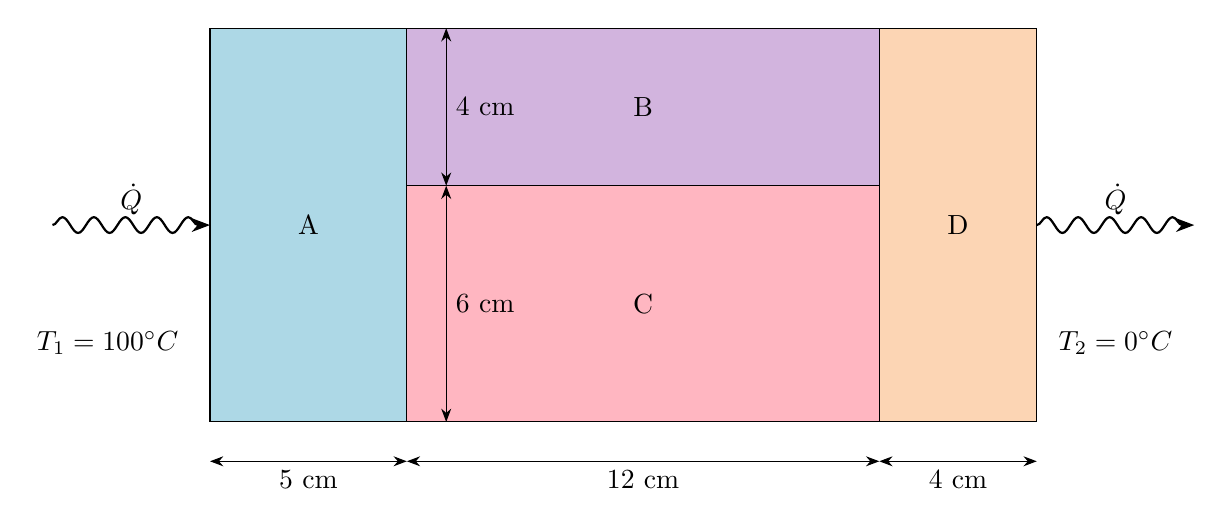
\begin{tikzpicture}[scale=0.5, >=Stealth]
% Define nodes for the temperatures
\node (T1) at (-2.6,2) {\(T_1 = 100^\circ C\)};
\node (T2) at (23,2) {\(T_2 = 0^\circ C\)};

% Draw the composite wall
\draw[fill=bluecolor] (0,0) rectangle (5,10); % Material A
\draw[fill=purplecolor] (5,6) rectangle (17,10); % Material B
\draw[fill=pinkcolor] (5,0) rectangle (17,6); % Material C
\draw[fill=orangecolor] (17,0) rectangle (21,10); % Material D

% Labels for materials
\node at (2.5,5) {A};
\node at (11,8) {B};
\node at (11,3) {C};
\node at (19,5) {D};

% Dimensions
\draw[<->] (0,-1) -- node[below] {5 cm} (5,-1);
\draw[<->] (5,-1) -- node[below] {12 cm} (17,-1);
\draw[<->] (17,-1) -- node[below] {4 cm} (21,-1);
\draw[<->] (6,6) -- node[right] {4 cm} (6,10);
\draw[<->] (6,0) -- node[right] {6 cm} (6,6);

% Heat flow arrows
\draw[->, thick, decorate, decoration={snake, amplitude=1mm, segment length=4mm, post length=1mm}] (-4,5) -- (0,5) node[midway,above] {\(\dot{Q}\)};
\draw[->, thick, decorate, decoration={snake, amplitude=1mm, segment length=4mm, post length=1mm}] (21,5) -- (25,5) node[midway,above] {\(\dot{Q}\)};
\end{tikzpicture}
\end{center}

\subsection*{Solution}
The thermal resistance for each material layer is given by the formula:
\[ R = \frac{L}{kA} \]
\noindent
For the given materials, we have:

\begin{itemize}
    \item Material A: \( k_A = 1 \, \text{W/(m}\cdot\text{K)} \), \( L_A = 0.05 \, \text{m} \), \( A_A = 0.1 \, \text{m}^2 \)
    \item Material B: \( k_B = 0.2 \, \text{W/(m}\cdot\text{K)} \), \( L_B = 0.12 \, \text{m} \), \( A_B = 0.04 \, \text{m}^2 \)
    \item Material C: \( k_C = 0.6 \, \text{W/(m}\cdot\text{K)} \), \( L_C = 0.12 \, \text{m} \), \( A_C = 0.06 \, \text{m}^2 \)
    \item Material D: \( k_D = 6 \, \text{W/(m}\cdot\text{K)} \), \( L_D = 0.04 \, \text{m} \), \( A_D = 0.1 \, \text{m}^2 \)
\end{itemize}
\noindent
Using the above formula, we calculate the thermal resistance for each material:

\begin{align*}
R_A &= \frac{0.05 \, \text{m}}{1 \, \text{W/(m}\cdot\text{K)} \times 0.1 \, \text{m}^2} \\
R_B &= \frac{0.12 \, \text{m}}{0.2 \, \text{W/(m}\cdot\text{K)} \times 0.04 \, \text{m}^2} \\
R_C &= \frac{0.12 \, \text{m}}{0.6 \, \text{W/(m}\cdot\text{K)} \times 0.06 \, \text{m}^2} \\
R_D &= \frac{0.04 \, \text{m}}{6 \, \text{W/(m}\cdot\text{K)} \times 0.1 \, \text{m}^2}
\end{align*}

Since materials B and C are in parallel, we find their combined resistance, \( R_{BC} \), using the formula for parallel resistances:

\[ \frac{1}{R_{BC}} = \frac{1}{R_B} + \frac{1}{R_C} \]
\noindent
The total thermal resistance of the wall, \( R_{\text{total}} \), is then the sum of the resistances in series:

\[ R_{\text{total}} = R_A + R_{BC} + R_D \]

\begin{center}
\begin{circuitikz}[american resistors, thick]
\tikzstyle{every node}=[font=\large]
% Defining the thermal resistances
\draw (0,-1) to[R, l=$A$, -*] (3,-1) 
      (3,0) to[short] (3,-2)
      (3,-2) to[R, l=$B$, -] (7,-2)
      (3,0) to[R, l=$C$, -] (7,0)
      (7,0) to[short] (7,-2)
      (7,-1) to[R, l=$D$, *-] (10,-1);

% Adding the input and output labels
\node at (-0.8,-1) {Input};
\node at (11,-1) {Output};
\end{circuitikz}
\end{center}

\subsubsection*{Heat Transfer Rate Calculation}

With the total thermal resistance and the temperature difference (\( \Delta T = 100 \, \text{K} \)), the heat transfer rate through the composite wall is calculated as:

\[ \dot{Q} = \frac{\Delta T}{R_{\text{total}}} \]

Plugging in the values from the thermal resistance calculations, we find the rate of heat transfer to be approximately \( 30.36 \, \text{W} \). This indicates that under the given conditions, around \( 30.36 \, \text{W} \) of heat will flow from the hot side (100°C) to the cold side (0°C) of the composite wall.
\newpage

\section*{Question \#5}
A furnace wall consists of a 0.3 m-thick inner layer of fire-clay brick (\(k = 1.7 \, \text{W/m}\cdot\text{K}\)), a 0.2 m-thick layer of kaolin brick (\(k = 0.12 \, \text{W/m}\cdot\text{K}\)), and a 0.1 m-thick outer layer of face brick (\(k = 1.3 \, \text{W/m}\cdot\text{K}\)). The temperature of the furnace gases is \(1400 \, \text{K}\), and the ambient air temperature is \(310 \, \text{K}\). The heat transfer coefficients on the inside and outside of the wall are \(100 \, \text{W/m}^2\text{K}\) and \(15 \, \text{W/m}^2\text{K}\), respectively.

\begin{enumerate}
    \item Determine the heat loss through a 4 m-high, 8 m-long wall.
    \item Determine the temperature of the external brick of the wall.
    \item If the external brick temperature should not exceed \(320 \, \text{K}\), determine how thick the Kaolin brick layer should be to achieve this condition.
\end{enumerate}
\begin{center}

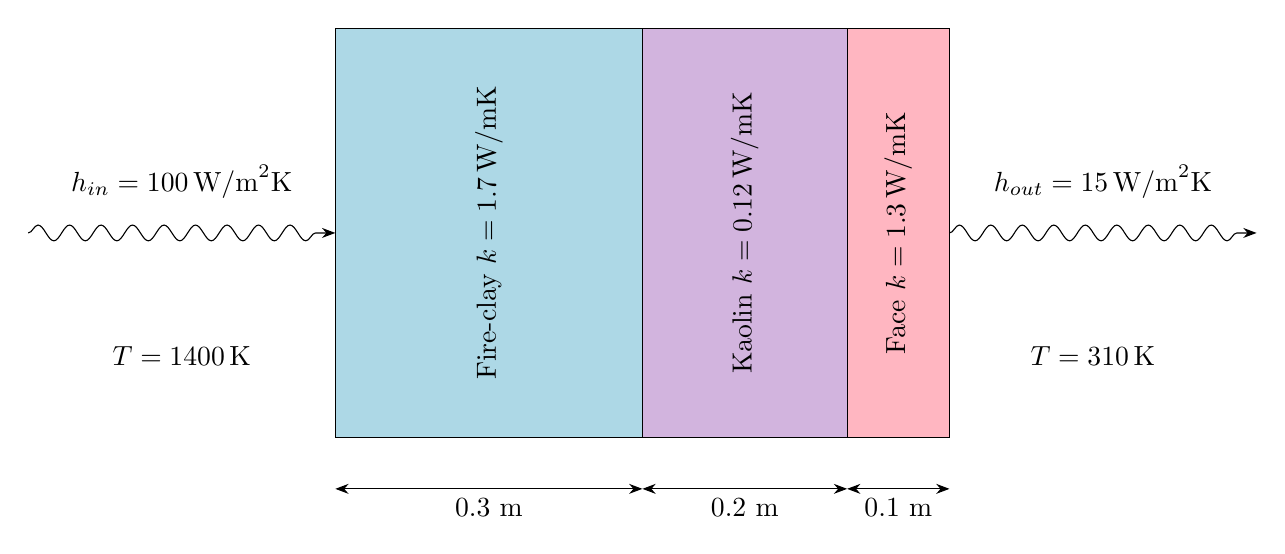
\begin{tikzpicture}[scale=1.3, >=Stealth]

% Define the layers with their thicknesses and thermal conductivities
\def\fireclay{3}
\def\kaolin{2}
\def\facebrick{1}
\def\wallheight{4}

% Fire-clay brick layer
\draw[fill=bluecolor] (0,0) rectangle (\fireclay,\wallheight) node[midway, rotate=90] {Fire-clay $k=1.7 \, \text{W/mK}$};

% Kaolin brick layer
\draw[fill=purplecolor] (\fireclay,0) rectangle (\fireclay+\kaolin,\wallheight) node[midway, rotate=90] {Kaolin $k=0.12 \, \text{W/mK}$};

% Face brick layer
\draw[fill=pinkcolor] (\fireclay+\kaolin,0) rectangle (\fireclay+\kaolin+\facebrick,\wallheight) node[midway, rotate=90] {Face $k=1.3 \, \text{W/mK}$};

% Inside heat transfer coefficient
\draw[->, decorate, decoration={snake, amplitude=1mm, segment length=4mm, post length=1mm}] (-3,\wallheight/2) -- (0,\wallheight/2);
\node at (-1.5,\wallheight/2+0.5) {$h_{in}=100 \, \text{W/m}^2\text{K}$};
\node at (-1.5,\wallheight/2-1.2) {$T=1400 \, \text{K}$} ;

% Outside heat transfer coefficient

% Wavy line
\draw[->, decorate, decoration={snake, amplitude=1mm, segment length=4mm, post length=1mm}] (6,\wallheight/2) -- (9,\wallheight/2);

\node at (7.5,\wallheight/2+0.5) {$h_{out}=15 \, \text{W/m}^2\text{K}$};
\node at (7.4,\wallheight/2-1.2) {$T=310 \, \text{K}$} ;
 
% Dimensions
\draw[<->] (0,-0.5) -- node[below] {0.3 m} (\fireclay,-0.5);
\draw[<->] (\fireclay,-0.5) -- node[below] {0.2 m} (\fireclay+\kaolin,-0.5);
\draw[<->] (\fireclay+\kaolin,-0.5) -- node[below] {0.1 m} (\fireclay+\kaolin+\facebrick,-0.5);

\end{tikzpicture}
\end{center}


\subsection*{Solution}
\begin{align*}
L_1 &= 0.3 \, \text{m} \\
k_1 &= 1.7 \, \text{W/m·K} \\
L_2 &= 0.2 \, \text{m} \\
k_2 &= 0.12 \, \text{W/m·K} \\
L_3 &= 0.1 \, \text{m} \\
k_3 &= 1.3 \, \text{W/m·K} \\
h_{\text{in}} &= 100 \, \text{W/m}^2\text{K} \\
h_{\text{out}} &= 15 \, \text{W/m}^2\text{K} \\
T_{\text{furnace}} &= 1400 \, \text{K} \\
T_{\text{ambient}} &= 310 \, \text{K} \\
A &= 32 \, \text{m}^2
\end{align*}
\noindent
Calculate resistances with numerical values:
\begin{align*}
R_{\text{conv, in}} &= \frac{1}{h_{\text{in}} \cdot A} = \frac{1}{100 \cdot 32} = 0.0003125 \, \text{m}^2\text{K/W} \\
R_{\text{conv, out}} &= \frac{1}{h_{\text{out}} \cdot A} = \frac{1}{15 \cdot 32} = 0.0020833 \, \text{m}^2\text{K/W} \\
R_{\text{cond, 1}} &= \frac{L_1}{k_1 \cdot A} = \frac{0.3}{1.7 \cdot 32} = 0.0055147 \, \text{m}^2\text{K/W} \\
R_{\text{cond, 2}} &= \frac{L_2}{k_2 \cdot A} = \frac{0.2}{0.12 \cdot 32} = 0.0520833 \, \text{m}^2\text{K/W} \\
R_{\text{cond, 3}} &= \frac{L_3}{k_3 \cdot A} = \frac{0.1}{1.3 \cdot 32} = 0.0024038 \, \text{m}^2\text{K/W}
\end{align*}
\noindent
Total thermal resistance:
\begin{align*}
R_{\text{total}} &= R_{\text{conv, in}} + R_{\text{cond, 1}} + R_{\text{cond, 2}} + R_{\text{cond, 3}} + R_{\text{conv, out}} \\
&= 0.0003125 + 0.0055147 + 0.0520833 + 0.0024038 + 0.0020833 \\
&= 0.0623976 \, \text{m}^2\text{K/W}
\end{align*}
\noindent
Heat transfer through the wall (\(Q\)) calculation with numerical values:
\[ Q = \frac{T_{\text{furnace}} - T_{\text{ambient}}}{R_{\text{total}}} = \frac{1400 - 310}{0.0623976} \approx 17468.59 \, \text{W} \]
\noindent
To find the external wall temperature (\(T_{\text{ext}}\)), calculate the temperature drop across each resistance and subtract from the furnace temperature:
\begin{align*}
\Delta T_{\text{conv, in}} &= Q \cdot R_{\text{conv, in}} = 17468.59 \cdot 0.0003125 = 5.46 \, \text{K} \\
\Delta T_{\text{cond, 1}} &= Q \cdot R_{\text{cond, 1}} = 17468.59 \cdot 0.0055147 = 96.33 \, \text{K} \\
\Delta T_{\text{cond, 2}} &= Q \cdot R_{\text{cond, 2}} = 17468.59 \cdot 0.0520833 = 909.82 \, \text{K} \\
\Delta T_{\text{cond, 3}} &= Q \cdot R_{\text{cond, 3}} = 17468.59 \cdot 0.0024038 = 41.99 \, \text{K} \\
T_{\text{ext}} &= T_{\text{furnace}} - (\Delta T_{\text{conv, in}} + \Delta T_{\text{cond, 1}} + \Delta T_{\text{cond, 2}} + \Delta T_{\text{cond, 3}}) \\
&= 1400 - (5.46 + 96.33 + 909.82 + 41.99) \\
&= 346.39 \, \text{K}
\end{align*}

\noindent
Given constants are the furnace internal temperature (\(T_{\text{furnace}} = 1400 \, \text{K}\)), the ambient temperature (\(T_{\text{ambient}} = 310 \, \text{K}\)), and the initial heat transfer rate (\(Q = 17468.59 \, \text{W}\)).
\newline

\textbf{Step 1: Initialization.} Start with an initial guess for the thickness of the kaolin brick, \(L_2\), based on standard values or previous calculations.
\newline

\textbf{Step 2: Resistance Calculation.} For the current thickness \(L_2\), compute the thermal resistance of the kaolin brick (\(R_{\text{cond, 2}}\)), and subsequently, the total thermal resistance (\(R_{\text{total}}\)) of the wall.
\newline

\textbf{Step 3: Heat Transfer and Temperature Calculation.} Utilizing the updated \(R_{\text{total}}\), recalculate the heat transfer rate (\(Q\)) through the wall and the resulting external temperature (\(T_{\text{ext}}\)) using the equation \(T_{\text{ext}} = T_{\text{furnace}} - Q \cdot (R_{\text{total}} - R_{\text{conv, out}})\).
\newline

\textbf{Step 4: Iteration.} Adjust \(L_2\) iteratively, employing the bisection method to minimize the difference between \(T_{\text{ext}}\) and the target temperature of \(320 \, \text{K}\).
\newline

\textbf{Step 5: Convergence.} The iteration proceeds until the calculated \(T_{\text{ext}}\) satisfactorily approaches \(320 \, \text{K}\) within a predefined tolerance level, indicating convergence.
\newline

\textbf{Step 6: Result.} Upon convergence, the algorithm yields the optimized thickness \(L_2\) of the kaolin brick, ensuring that \(T_{\text{ext}} \leq 320 \, \text{K}\). The thickness was found to be \textbf{0.83239276 meters}.

The Heat Loss was also found to be \textbf{4800 W} via the algorithm above.

\end{document}
